\newcommand{\ClassPath}{../../VIU_TFM_LaTeX_template}
\documentclass{\ClassPath/viu-tfm-template}
\usepackage{multicol}

\definecolor{maincolor}{HTML}{f25416}

%--------------------------------------------------------------------------
% Definiciones necesarias Modifica con tus datos
%--------------------------------------------------------------------------
\def\nombre{Gómez Olivencia, Rubén}
\def\dni{78910013-A}
\def\titulo{JAWC \linebreak\linebreak (\textit{just another wordle clone}) \linebreak\linebreak creado en Angular}
\def\titulacion{Máster Universitario en Desarrollo de Aplicaciones y Servicios Web}
\def\curso{2022-2023}

%Los siguientes son opcionales: si no se ponen, la portada cambia un poco. Ideal para escribir artículos/trabajos cortos
\def\dirige{}
\def\convocatoria{}
\def\asignatura{Desarrollo de aplicaciones web II: lado del cliente (front-end) y multimedia}


% importar fichero de Bibliografía
%\addbibresource{Actividad_1.bib}

\begin{document}
    \graphicspath{{../../VIU_TFM_LaTeX_template/}}

    \coverpage

    \tableofcontents

\chapter{Introducción}

\href{https://www.nytimes.com/games/wordle/index.html}{Wordle} es un juego  que ha adquirido bastante fama debido a su sencillez, pero que al mismo tiempo tiene una mecánica adictiva: tratar de adivinar una palabra en un número máximo de intentos.

A lo largo de este documento se va a explicar cómo se ha realizado un “clon” del juego, habiendo decidido ampliar las posibilidades del juego.

Para realizar este desarrollo se ha hecho uso del \textit{framework} de \textit{front-end} \href{https://angular.io/}{Angular}, que hace uso del lenguaje de programación \href{https://www.typescriptlang.org/}{Typescript}, y para dar un aspecto visual más cuidado se ha utilizado el \textit{framework} de estilos \href{https://getbootstrap.com/}{Bootstrap}.

\chapter{Objetivo del desarrollo}

Como ya se ha comentado, el objetivo ha sido desarrollar un clon del juego, tratando de mantener las características que todos los usuarios del original conocen, pero añadiendo opciones nuevas. Los objetivos iniciales eran:

\vspace{-1em}
\begin{itemize}
    \item Crear funcionalidades básicas del juego original.
    \item Confirmar que el juego funciona en dispositivos móviles gracias al interfaz \textit{responsive}.
    \item Añadir nuevas opciones de juego:
    \begin{itemize}
        \item Poder elegir el número de intentos para acertar la palabra.
        \item Poder elegir la longitud de las palabras a adivinar.
    \end{itemize}
\end{itemize}
\vspace{-1em}

De esta manera, se ha tratado de realizar un juego fácilmente ampliable de cara a futuro, y que el usuario pueda elegir su nivel de dificultad.


\chapter{Desarrollo realizado}
Tal como se ha indicado previamente, para realizar este proyecto se ha utilizado \href{https://angular.io/}{Angular} como \textit{framework} de desarrollo. Esto nos ha permitido realizar un desarrollo auto-contenido que se puede convertir en una aplicación \textit{standalone} ya que, en este caso, no es necesario hacer uso de servicios externos.


\begin{center}
    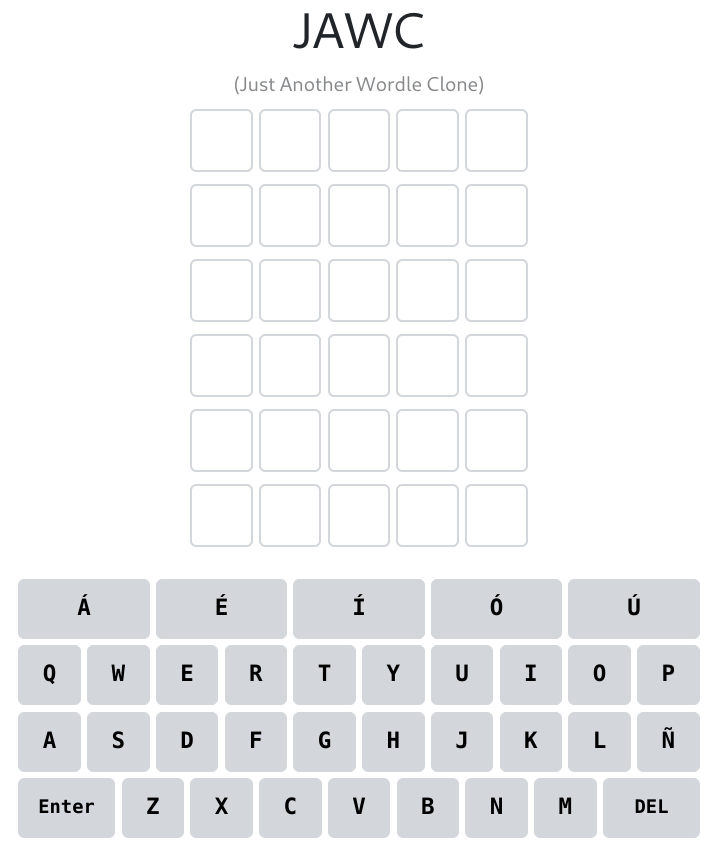
\includegraphics[frame,width=0.7\linewidth]{img/inicio.png}
\end{center}

El juego hace uso dos componentes distintos, correspondientes a las vistas de:

\vspace{-1em}
\begin{itemize}
    \item \textbf{Letras}: Cada letra es una instancia de un componente. En este componente lo que hace es controlar el color que debe de tener la letra. Para ello se recibe un parámetro del componente padre.
    \item \textbf{Teclado}: Todo el teclado es un componente separado, que realiza una función similar a las letras. Recibe como parámetro el estado que debe tener para que se muestren del color correspondiente.
\end{itemize}
\vspace{-1em}

De esta manera, toda la lógica del juego se realiza en el componente principal \textit{App}, y se llama a los hijos con los parámetros necesarios para que actualicen su estado y por tanto modifiquen su vista.

\section{Características básicas}
A continuación se van a detallar las características básicas y cómo se han realizado.

\subsection{Diccionario}
El juego se basa en acertar palabras, por lo que lo primero era conseguir un diccionario para las palabras a utilizar. El desarrollo se ha realizado bajo \textbf{GNU/Linux}, y todas las distribuciones cuentan con diccionarios para poder realizar las correcciones en los editores de texto: Es por eso que se ha podido utilizar el siguiente comando para obtener las palabras:

\begin{mycode}{Obtención de las palabras de 5 letras del diccionario}{bash}{}
grep -E '^[[:alpha:]]{5}$' /usr/share/dict/spanish > /tmp/5
\end{mycode}

De esta manera se han obtenido todas las palabras de cinco letras del diccionario en un fichero, siendo cada línea una palabra. Una vez hecho eso, ha sido suficiente con añadir comillas y una coma al final de la palabra para poder convertirlo en un array para usarlo. Aparte, se han creado dos funciones para interactuar con el diccionario que se encuentra en \configfile{src/assets/js/dictionary.js}.

\subsection{Comprobar la palabra introducida}
Con el diccionario ya formado, el siguiente paso era comprobar si la palabra introducida por el usuario coincidía con la palabra elegida aleatoriamente y realizar el cambio de color.

\vspace{-1em}
\begin{center}
    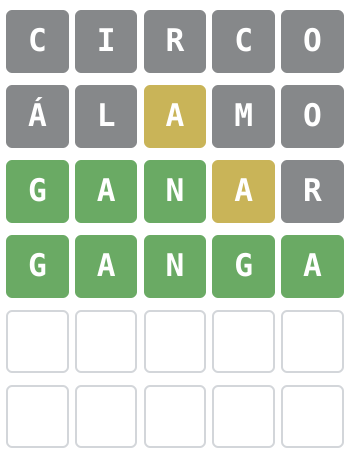
\includegraphics[width=0.3\linewidth]{img/juego1.png}
\end{center}
\vspace{-1em}

Durante los primeros pasos del desarrollo, para introducir la palabra se hacía uso de un \textit{textinput}. Esto facilitó centrarse en el algoritmo principal y la parte funcional del juego, dejando el aspecto visual final para más adelante.

Estas versiones previas del juego se pueden visualizar en el repositorio de \href{https://github.com/yuki/jawc}{Github donde está alojado el proyecto}.

Para facilitar el \textit{debug} del juego, todavía se mantiene el comando que saca la palabra que hay que adivinar \inlineconsole{console.log(this.word)} y se puede ver en las “herramientas del desarrollador” al comenzar el juego.

\subsection{Aspecto visual}
El juego original es bastante simple a nivel visual, pero eso no quita que haya retos detrás de él, ya que la visualización debe ser correcta también en dispositivos móviles.

\vspace{-1em}
\begin{center}
    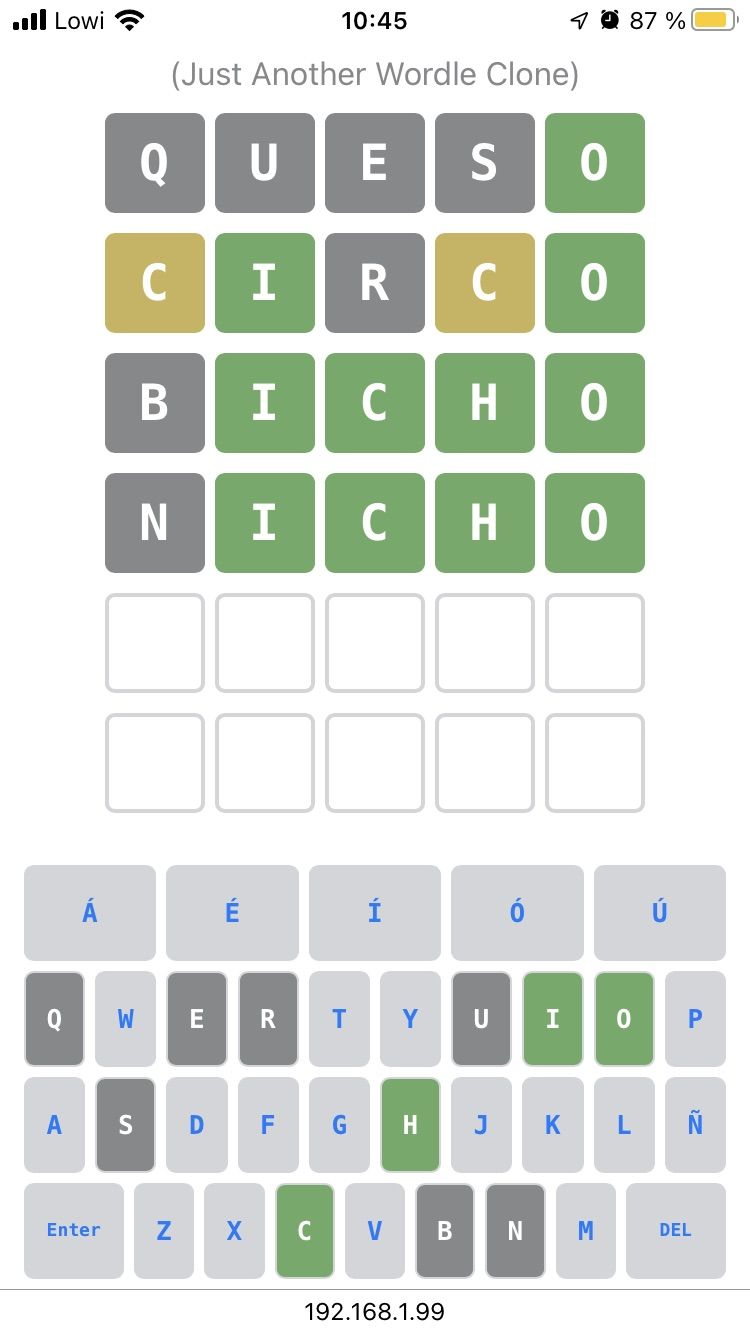
\includegraphics[frame,width=0.48\linewidth]{img/movil.png}
\end{center}
\vspace{-1em}

Durante el desarrollo ha habido algunas modificaciones en el aspecto, ya que inicialmente se buscaba que funcionase antes que la eficiencia.

Al finalizar el desarrollo, la parte superior se ha realizado haciendo uso de \textit{div}s y el sistema \textbf{\textit{grid}} de CSS, para formar una cuadrícula perfecta, mientras que para el teclado se han utilizado botones cuyo aspecto ha sido modificado para que se ajusten al tamaño del dispositivo.


\subsection{Error con palabras no válidas}
Aparte, cuando el usuario introduce una palabra, esta se comprueba contra el diccionario existente. De no existir, el usuario recibirá un error, no se contará el intento y por tanto deberá borrar la palabra para introducir una válida.

\vspace{-1em}
\begin{center}
    
\includegraphics[width=0.7\linewidth]{img/error.png}
\end{center}
\vspace{-1em}

Es cierto que este aviso no aparecía en un primer momento, ni se realizaba la comprobación, ya que se decidió posponer esta característica al final del desarrollo ya que era sencillo de realizar y se prefería centrar el esfuerzo en otros aspectos.


\section{Nuevas características}
Como se ha dicho al inicio del documento, desde el inicio del desarrollo se quería ampliar las opciones del juego original, y para ello al iniciar el juego se ha introducido un pequeño menú en el que nos deja elegir dos aspectos del juego:

\vspace{-1em}
\begin{center}
    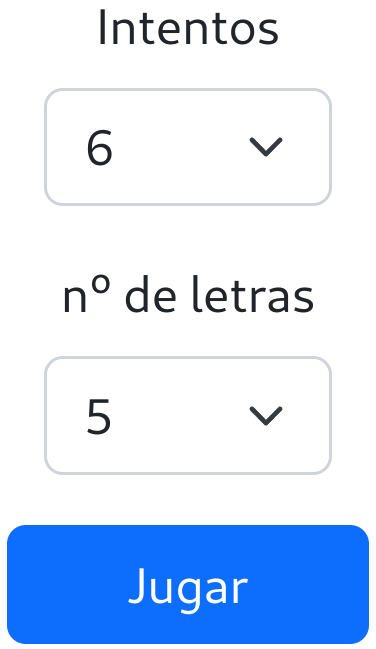
\includegraphics[width=0.2\linewidth]{img/opciones.png}
\end{center}
\vspace{-1em}

Las opciones hacen referencia a:
\vspace{-1em}
\begin{itemize}
    \item \textbf{Número de intentos}: En el juego original sólo se permiten 6 intentos para conseguir acertar la palabra. A modo de poder elegir el nivel de dificultad, en esta versión se permite elegir cuántos intentos vamos a poder utilizar, entre 3 y 12.
    \item \textbf{Número de letras}. De nuevo, el juego original está limitado a palabras de cinco letras, lo que puede resultar en poca variedad. Es por eso que se ha decidido ampliar las opciones dando la opción de elegir jugar con palabras de entre 4 y 7 letras.
\end{itemize}
\vspace{-1em}

De esta manera podemos tener más posibilidades a la hora de jugar, como el siguiente ejemplo de 4 intentos para palabras de 6 letras:

\vspace{-1em}
\begin{center}
    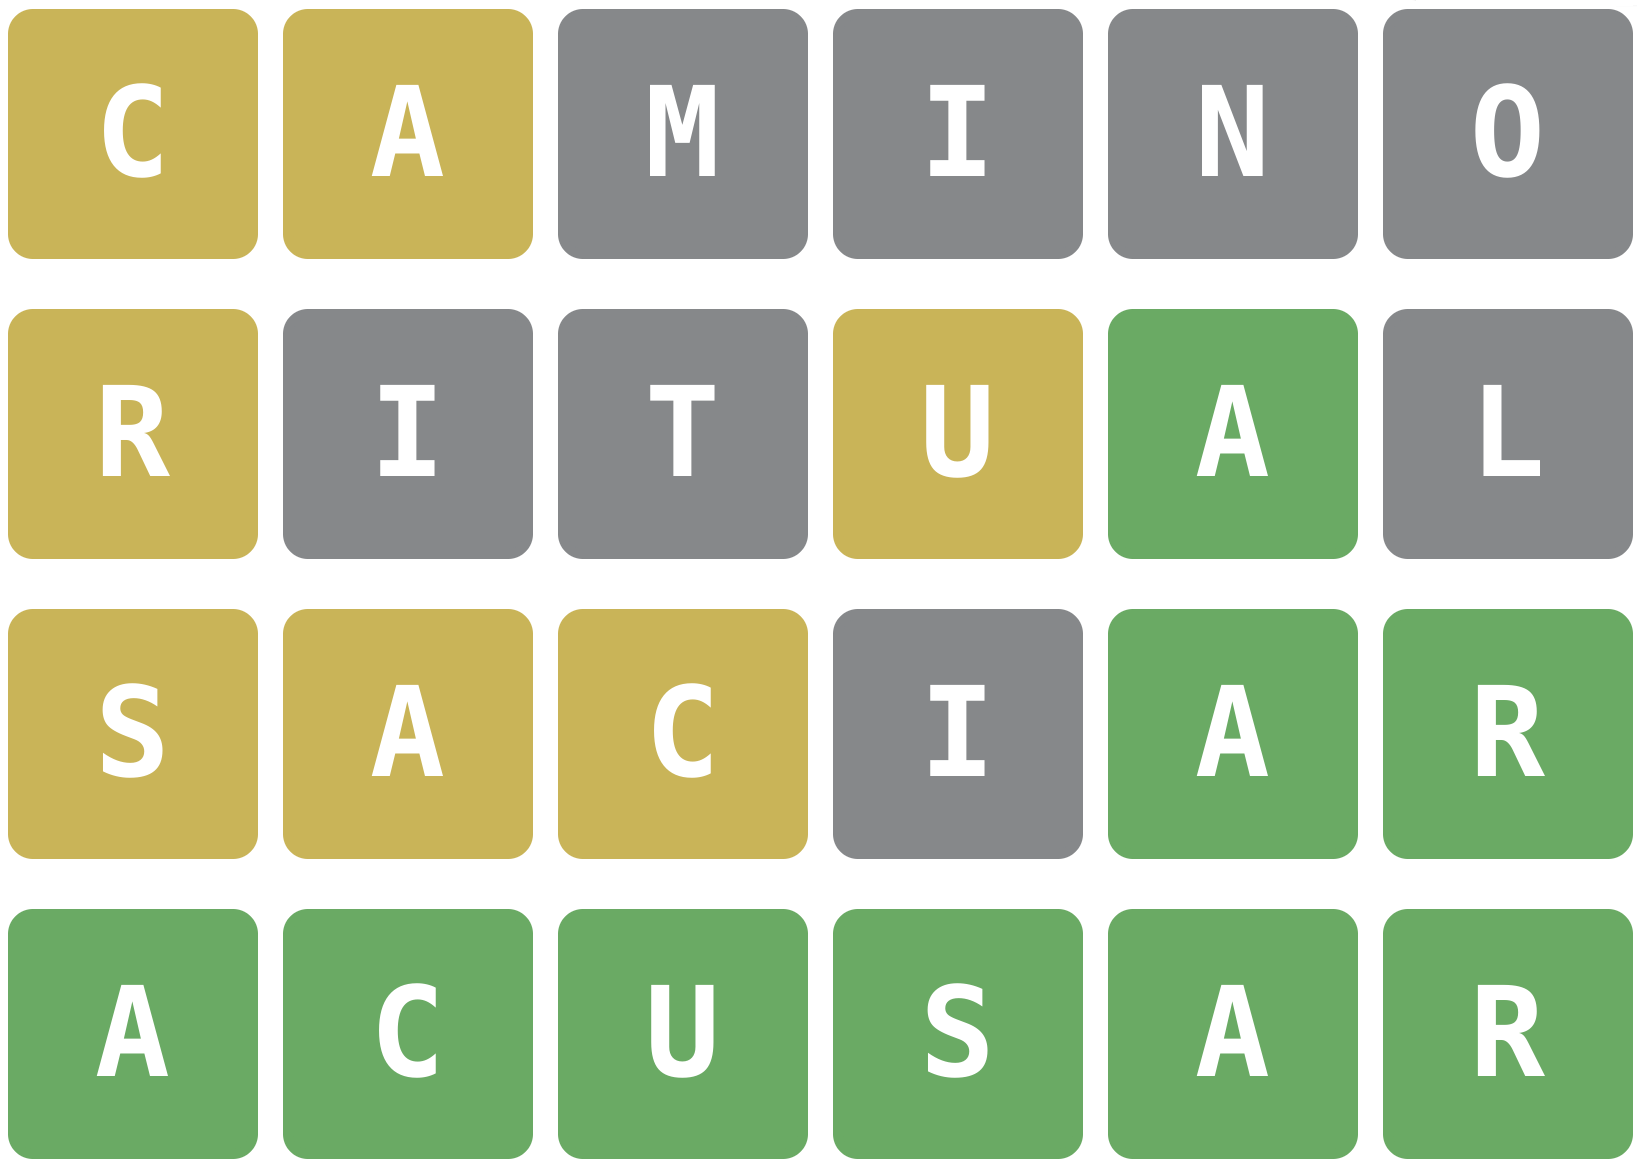
\includegraphics[width=0.4\linewidth]{img/6letras.png}
\end{center}
\vspace{-1em}


\subsection{Despliegue automático de la aplicacón}
Dado que el desarrollo se ha utilizado haciendo uso de un repositorio en \href{https://github.com/yuki/jawc}{Github}, se ha aprovechado para realizar un \textit{action} que realiza el despliegue automático de los cambios realizados haciendo uso de las \textbf{Github Pages} dando lugar a que el juego pueda ser utilizado en la siguiente \href{https://yuki.github.io/jawc/}{URL}.

\vspace{-1em}
\begin{center}
    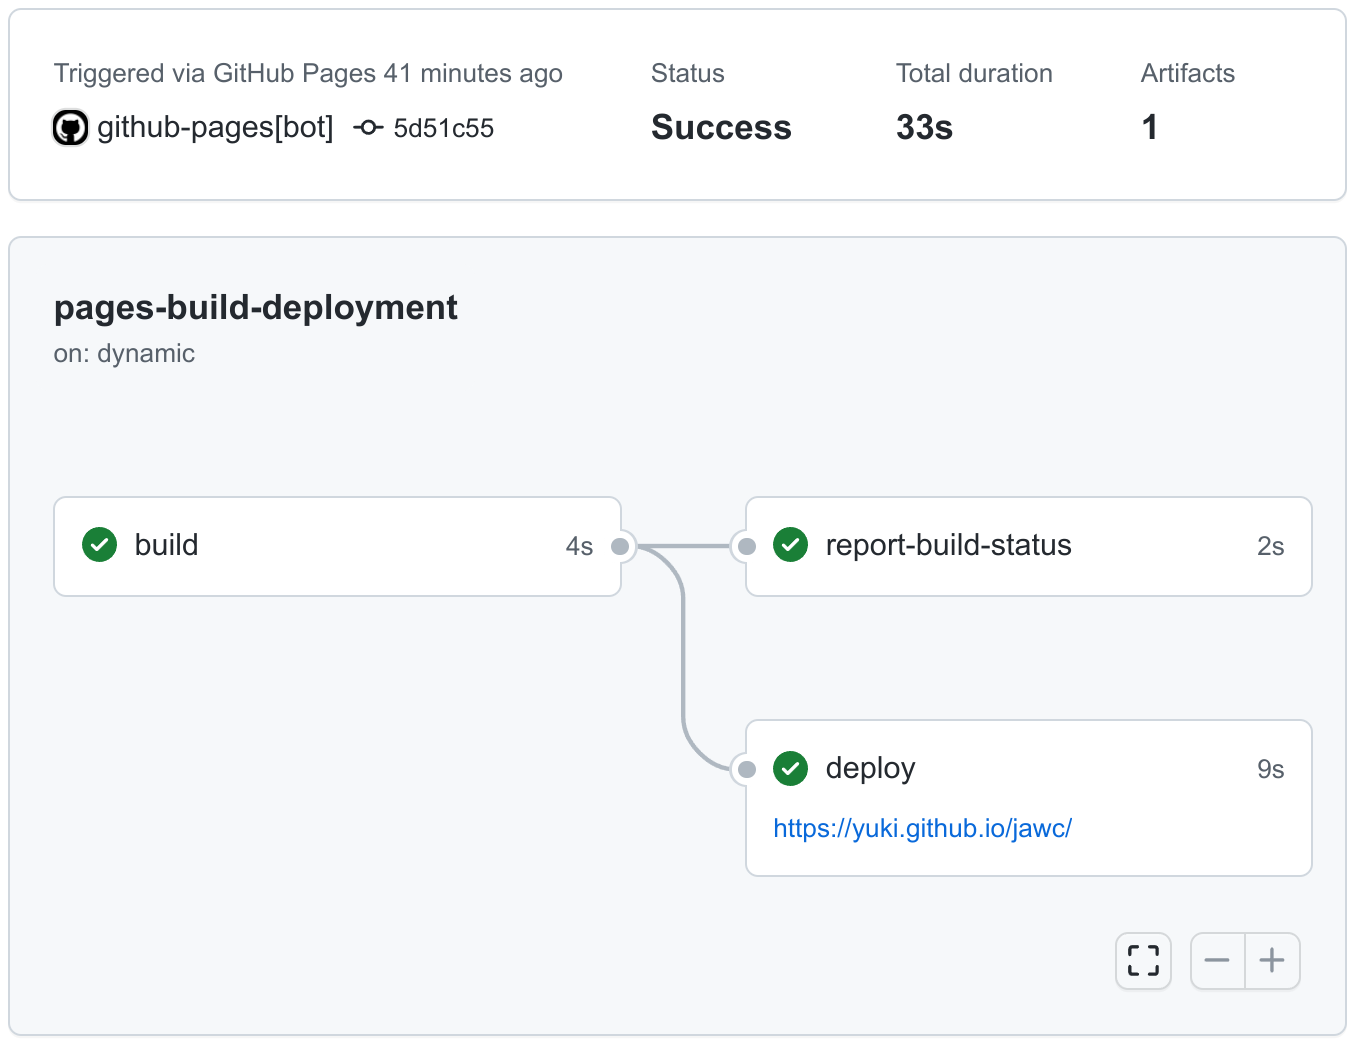
\includegraphics[width=0.7\linewidth]{img/deploy.png}
\end{center}
\vspace{-1em}

La configuración del despliegue se encuentra en el fichero de configuración  \configfile{.github/workflows/gh-pages.yml} situado en el repositorio.


\chapter{Dificultades del proyecto}

Como todo proyecto de programación, durante el desarrollo nos podemos encontrar con ciertas dificultades que deben ser subsanadas para llegar a cumplir los requisitos planteados al comienzo del proyecto.

La mecánica del juego es bastante sencilla, y se puede abordar desde distintos puntos de vista, pero el quid era cómo realizar el dibujado de las casillas donde se sitúan las letras, dependiendo de si existen o no en la palabra objetivo.

El desarrollo final cuenta con un array que se crea al iniciar la partida que consta de las siguientes dimensiones:

\vspace{-1em}
\begin{itemize}
    \item \textbf{Número de intentos}: La primera dimensión es el número de intentos que elige el usuario al iniciar la partida.
    \begin{itemize}
        \item \textbf{Número de letras}: Cada intento a su vez es un \textit{array} que tiene tantas posiciones como número de letras tiene la palabra a acertar. Cada letra, a su vez consta de un \textit{array} de dos posiciones donde las posiciones son:
        \begin{itemize}
            \item La \textbf{letra} introducida por el usuario.
            \item El \textbf{valor} de esa letra en la palabra a descubrir, que cuando se realiza la comprobación (al pulsar “intro”) tendrá uno de estos valores:
            \begin{itemize}
                \item \textbf{OK}: La letra existe en esta posición.
                \item \textbf{exists}: La letra existe en la palabra, pero en otra posición.
                \item \textbf{no}: La letra no existe en la palabra.
            \end{itemize}
        \end{itemize}
    \end{itemize}
\end{itemize}
\vspace{-1em}

De esta manera, la cuadrícula de intentos se dibuja teniendo en cuenta las dos primeras dimensiones de este \textit{array}, que llaman al componente \textbf{letra} pasando como parámetro el \textit{array} de cada letra (para que dibuje la propia letra y su estado).

Este array se actualiza cada vez que el usuario pulsa “intro”, lo que llama a la función \inlineconsole{check_word()} que realiza la comprobación de la palabra y actualiza el \textit{array}. Esto hace que cuando haya modificaciones, los componentes se actualizan.

Para dibujar el teclado virtual se hace de manera similar, pero en este caso sólo es necesario un \textit{array} de una dimensión que se va actualizando con las letras introducidas.


\chapter{Mejoras a realizar}
Aunque las funcionalidades básicas del proyecto están cumplidas, por falta de tiempo ha habido algunas características que no se han realizado y existen varias mejoras que se podrían realizar, siendo algunas de ellas:

\vspace{-1em}
\begin{itemize}
    \item \textbf{Efectos de las letras}: Cuando se valide la palabra, que las letras realicen el mismo efecto que en el juego original.

    \item \textbf{Guardar puntuación}: Para saber cuántas palabras seguidas se han acertado, se podrían guardar en el \textit{storage} del navegador un contador.

    \item \textbf{Letras con tilde}: Actualmente las letras con tilde sólo se pueden escribir desde el teclado virtual.

    \item \textbf{Compartir en redes sociales}: Al igual que el juego original, la posibilidad de compartir el resultado de la partida en distintas redes sociales.

    \item \textbf{Elección del idioma}: La posibilidad de añadir distintos idiomas al inicio de la partida es una opción que permitiría que el juego alcanzase más cuota de mercado.

    \item \textbf{Prescindir de Bootstrap}: El uso que se hace de la librería es mínimo, siendo el uso más importante la opción del “modal”.

    \item \textbf{Usar servicio externo para el diccionario}: Tal como se ha dicho, actualmente la aplicación es autocontenida, pero si se decidiese ampliar el diccionario esto repercutiría en el tamaño del mismo. Habría que valorar ventajas e inconvenientes de la decisión.
\end{itemize}
\vspace{-1em}


\chapter{Conclusiones}

Una vez más, una premisa sencilla pero bien ejecutada, y que resulta adictiva, hizo que \href{https://www.nytimes.com/games/wordle/index.html}{Wordle} se convirtiese en un juego jugado por millones de personas en todo el mundo.

En este caso, además, es fácilmente recreable tal como se ha realizado en este proyecto, y que permite, con ello, poder servir de estímulo para aprender un nuevo lenguaje de programación y \textit{framework} como son Typescript y Angular respectivamente.

Por todo ello ha resultado un proyecto interesante de realizar y que se tratará de añadir alguna de las mejoras propuestas tras la entrega del mismo.

\end{document}